\documentclass{article}


\usepackage{hyperref}
\usepackage{graphicx}
\usepackage{cite}


\hypersetup{
  pdfauthor={Matti Pastell},
  colorlinks=TRUE,
  linkcolor=black,
  citecolor=blue,
  urlcolor=blue
}


%Sivujen otsikot
\usepackage{fancyhdr}
\pagestyle{fancy}
\renewcommand{\sectionmark}[1]{%
\markright{\thesection\ #1}}
\fancyhf{} % delete current header and footer
\fancyhead[LE,RO]{\bfseries\thepage}
\fancyhead[LO]{\bfseries\rightmark}
\fancyhead[RE]{\bfseries\leftmark}
\renewcommand{\headrulewidth}{0.5pt}
\renewcommand{\footrulewidth}{0pt}
\addtolength{\headheight}{0.5pt} % space for the rule
\fancypagestyle{plain}{%
\fancyhead{} % get rid of headers on plain pages
\renewcommand{\headrulewidth}{0pt} % and the line
}

\newcommand{\HRule}{\rule{\linewidth}{0.5mm}}


% \usepackage{graphics}

%Ei sisennyst�
%\setlength\parindent{0in}

% ��kk�set
%\usepackage[utf8]{inputenc}
%\usepackage[T1]{fontenc}
%\usepackage{times}

\usepackage{Sweave}
\begin{document}

%\begin{titlepage}
%\ThisULCornerWallPaper{0.3}{logo}


%
\includegraphics[width=0.6\textwidth]{logo}\\[2cm]

\vspace*{1cm}
%\hspace{5cm}


\noindent \textsc{\Large Analyze Animal Behavior Data Using:}\\[0.1cm]
% Title
\HRule \\[0.2cm]
\begin{center}
{ \huge \bfseries Animal}\\[0.4cm]
\HRule \\[5cm]
\end{center}

%\vfill

\noindent \textsc{\Large Matti Pastell}\\[0.5cm]
\noindent \textsc{\Large Department of Agrotechnology \\[0.1cm] \& Research
  Center of Animal Welfare}\\[0.5cm]

%\noindent \url{http://www.mm.helsinki.fi/~mpastell}


%\AddToShipoutPicture{
\includegraphics[height=0.5\paperheight]{MMM}}
%\ThisLRCornerWallPaper{0.6}{MMM}

\end{titlepage}


%\begin{thebibliography}{9}
 % \bibitem{}
%\end{thebibliography}


\title{
\noindent \textsc{\Large Analyze Animal Behavior Data Using:}\\
% Title
\HRule \\
\begin{center}
{ \huge \bfseries Animal}\\
\HRule \\[0.2cm]
\end{center}
}

\author{
\Large Matti Pastell\\
\url{matti.pastell@helsinki.fi}\\[0.5cm]
Department of Agrotechnology \& \\
Center of Animal Welfare, \textit{University of Helsinki}
}

  % Matti Pastell \\ matti.pastell@helsinki.fi}

\maketitle




\section{Introduction}
The \texttt{Animal} package is a collection of functions for analyzing animal
behavior data originating from a variety of sources. The package was
originally created to analyze data files from CowLog (open source
software for coding behaviors from digital video), but the
functionality has been extended to cover also other data sources.
This document briefly describes some the key features of the package
via simple examples. \\
Animal has been created in the Research Centre of Animal Welfare
\footnote{\url{http://http://www.vetmed.helsinki.fi/hyvinvointikeskus/english/index.htm}}.


\section{CowLog data}
The package has basic analysis functions for analyzing time coded
behavioral data coded with CowLog\cite{cowlog}
\footnote{\url{http://www.mm.helsinki.fi/~mpastell/CowLog}}.
The main function in the package is \textit{cowAnalyze}. The function
takes the data file name, labels of the codes and the type (event or
state) of the codes as inputs, and gives a summary table and plot of
the results as output. The function also removes double state
(duplicated) errors for state codes.  

Here is a short example on how to use the function in R:
Analyze CowLog datafile named calf1.bh1: Define codes 1-3 and give them names walking, standing and lying. The descriptive statistics will appear on screen and they are also saved to variable analyzed.  
\begin{Schunk}
\begin{Sinput}
> library(Animal)
> analyzed <- cowAnalyze(file = "calf1.bh1", states = c(1, 
+     2, 3), state.names = c("walking", "standing", "lying"))
\end{Sinput}
\begin{Soutput}
Event results 	 
Frequency 	 0 times 
State results 	 walking standing lying 
Frequency 	 270 269 21 times 
Bout 		 0.8 0.37 54.98 minutes 
Total 		 214.81 99.35 1154.62 minutes 
\end{Soutput}
\end{Schunk}
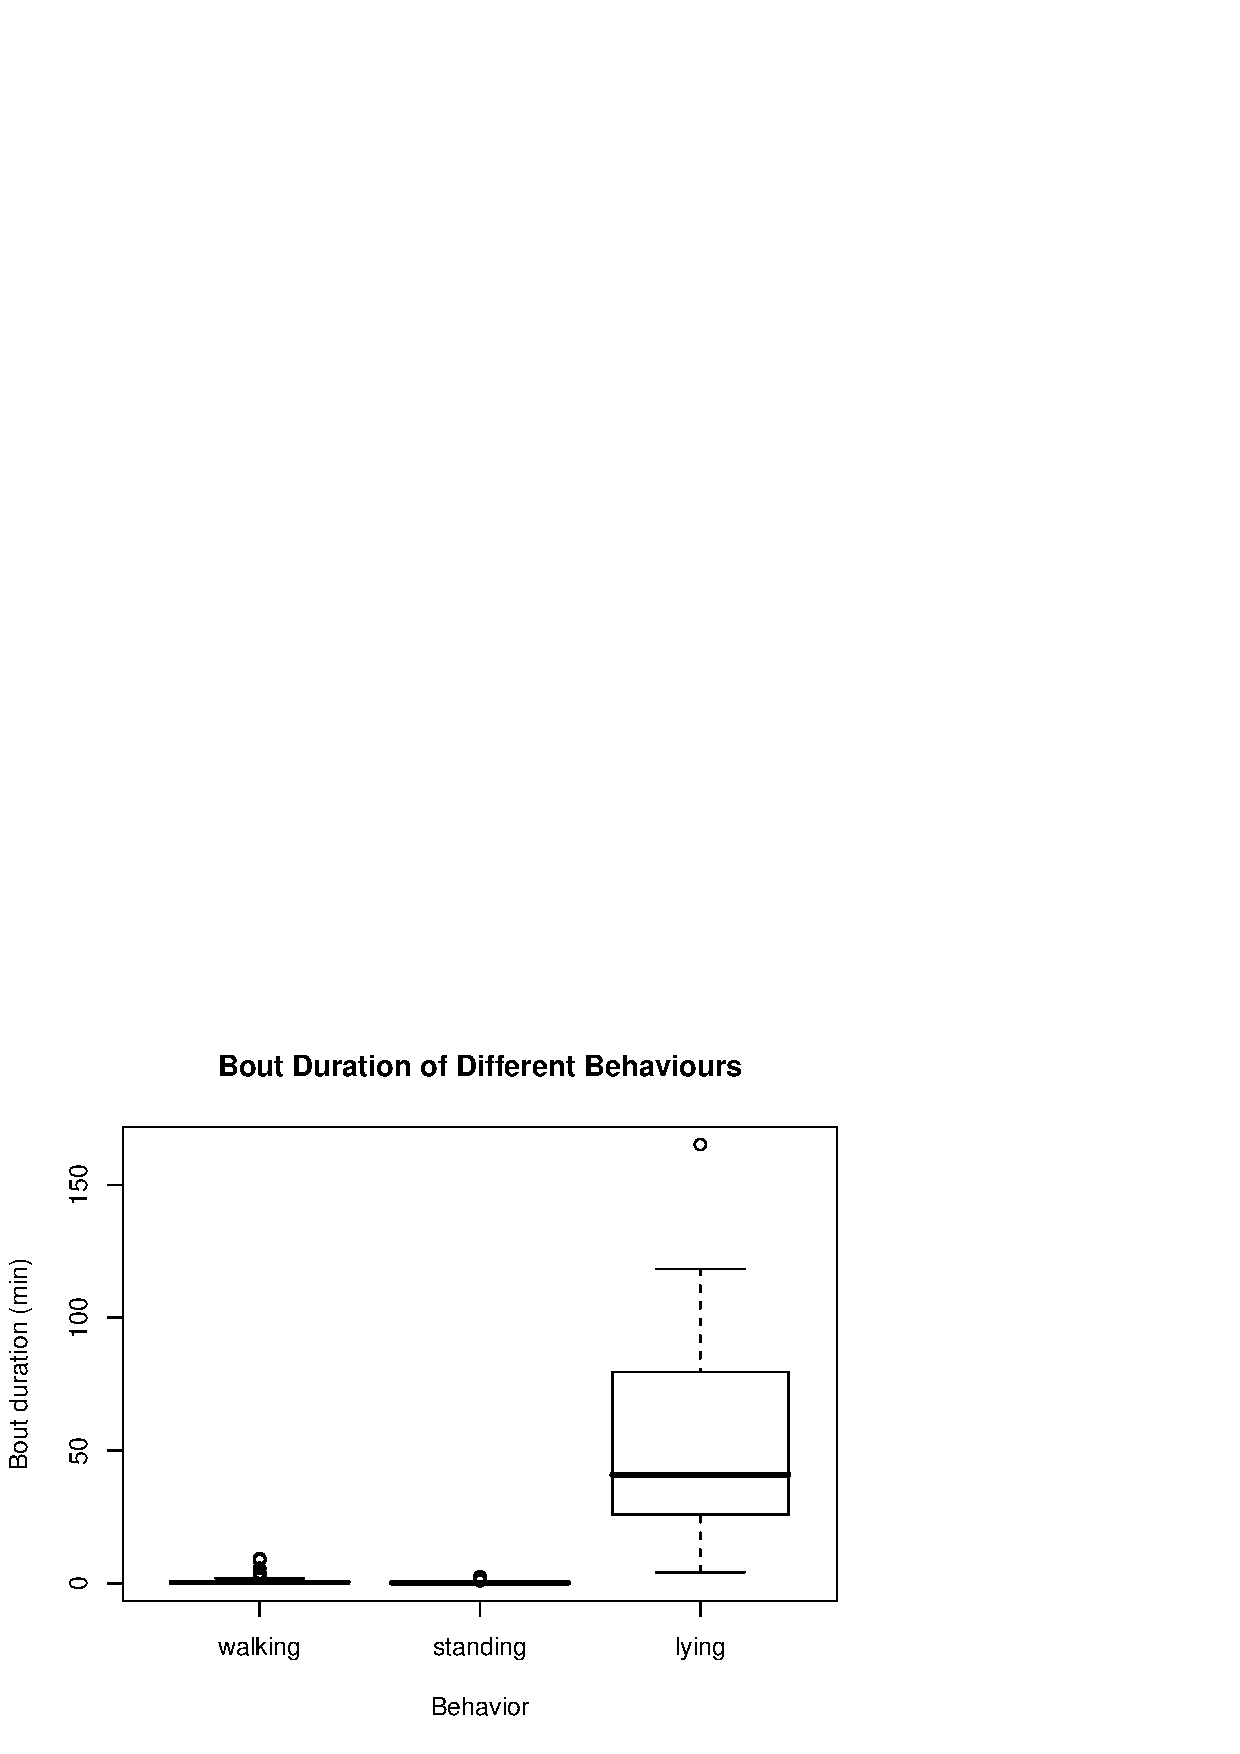
\includegraphics{Animal-002}
  

\section{RIC data}
The Animal package has several functions for working with the data
produced by Insentec RIC feed measurement system. The basic function
\texttt{read.RIC} can be used to read in RIC log files and they can be
processed using \texttt{clean.RIC} and \texttt{bouts.RIC} functions.

Example data has been read in by using read.RIC with option clean=F
It is included in the package as dataset RIC.
\begin{Schunk}
\begin{Sinput}
> data(RIC)
\end{Sinput}
\end{Schunk}

First we clean the data from zero rows and negative feed intakes, then
we merge the feeding bouts that are less than 5 minutes apart.

\begin{Schunk}
\begin{Sinput}
> RIC2 <- clean.RIC(RIC)
> bouts <- bouts.RIC(RIC2)
> head(bouts, 5)
\end{Sinput}
\begin{Soutput}
  cowID trough               begin                 end intake
1   320     11 2009-03-18 00:47:02 2009-03-18 01:12:03    4.8
2   320     11 2009-03-18 01:40:57 2009-03-18 01:51:53    2.6
3   320     11 2009-03-18 04:02:20 2009-03-18 04:22:30    2.9
4   320     11 2009-03-18 06:10:23 2009-03-18 07:24:27    9.8
5   320     11 2009-03-18 08:51:23 2009-03-18 08:56:11    1.0
  bout.duration intake.duration
1 25.01667 mins        24.51667
2 10.93333 mins        10.93333
3 20.16667 mins        15.81667
4 74.06667 mins        63.13333
5  4.80000 mins         4.80000
\end{Soutput}
\end{Schunk}
We can plot the feed intake distribution during different hours of the
day with the help of \texttt{partOfDay} function.

\begin{Schunk}
\begin{Sinput}
> boxplot(intake ~ partOfDay(begin), data = bouts, ylab = "Feed intake (kg)", 
+     xlab = "Time of day", main = "Default settings: start =1, nsplit=4")
\end{Sinput}
\end{Schunk}
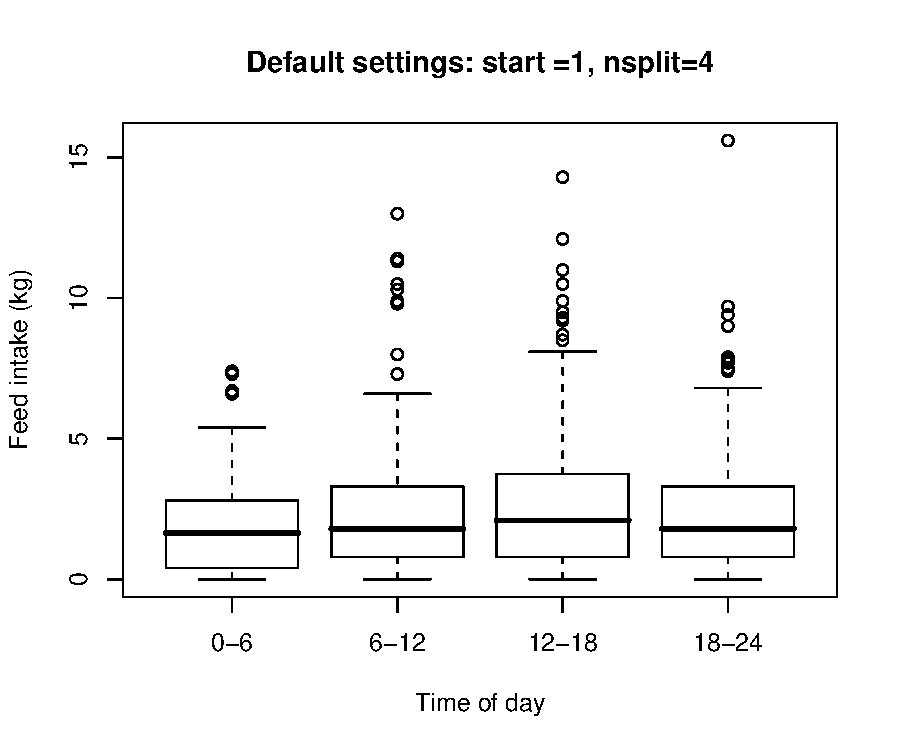
\includegraphics{Animal-005}

\section{Summarizing time series}
We are frequently interested in summarising events by an hour, day,
week or a month. Say how many times a cow has visited the feeding
trough during the day or what is the hourly sum of the feed intake for
each animal. Animal provides functions to calculate these things
easily with functions \texttt{hourly, daily, weekly and
  monthly}.\footnote{These are just simple wrapper functions to aggregate, but
I feel these are easier to remember and more convinient in frequent use}

The basic syntax for all functions is similar: We need to specify the
data vector we want to analyze, the time stamps for the data in
POSIXct format, the summarizing function and optionally the subject.

For instance, we are intersted in what is the hourly (\textit{summarized
according to the start time of feeding event}) number of visits in
the dataset \texttt{bouts} (created in RIC data chapter).

\begin{Schunk}
\begin{Sinput}
> attach(bouts)
> hourly.visits <- hourly(intake, begin, fun = length)
> head(hourly.visits)
\end{Sinput}
\begin{Soutput}
  Hour Result
1    1     35
2    2     33
3    3     37
4    4     29
5    5     22
6    6     21
\end{Soutput}
\begin{Sinput}
> plot(Result ~ Hour, data = hourly.visits, type = "b")
\end{Sinput}
\end{Schunk}
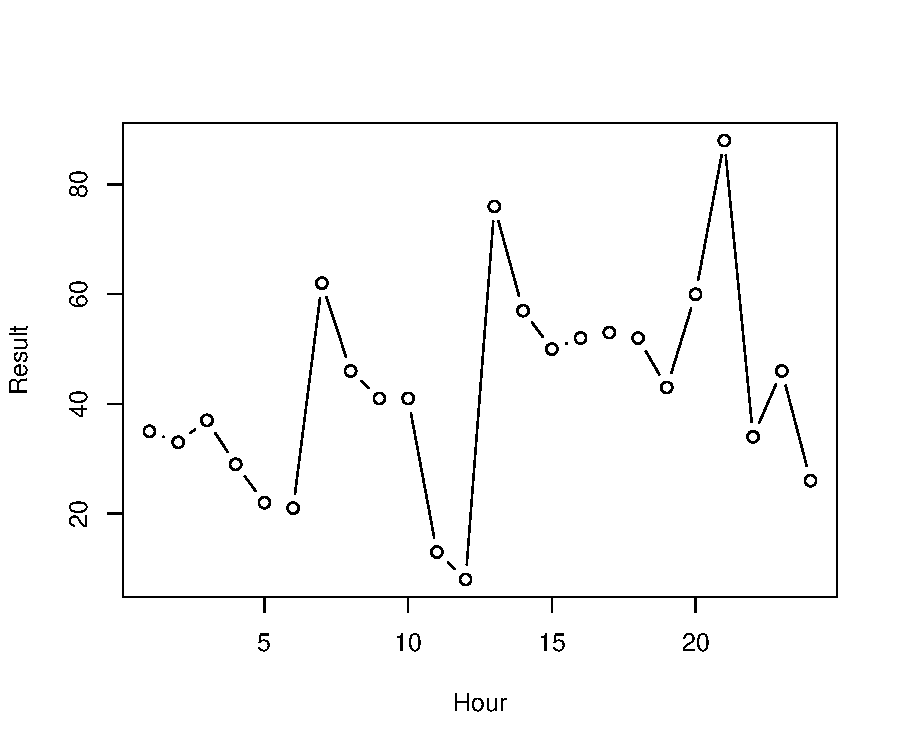
\includegraphics{Animal-006}

Similarly we can summarize the hourly intake for each cow:

\begin{Schunk}
\begin{Sinput}
> cow.intake <- hourly(intake, begin, fun = sum, subject = cowID)
> head(cow.intake)
\end{Sinput}
\begin{Soutput}
  Hour Subject Result
1    1     320    4.8
2    2     320    2.6
3    5     320    2.9
4    7     320    9.8
5    9     320    1.0
6   10     320    3.8
\end{Soutput}
\begin{Sinput}
> boxplot(Result ~ Hour, data = cow.intake)
> detach(bouts)
\end{Sinput}
\end{Schunk}
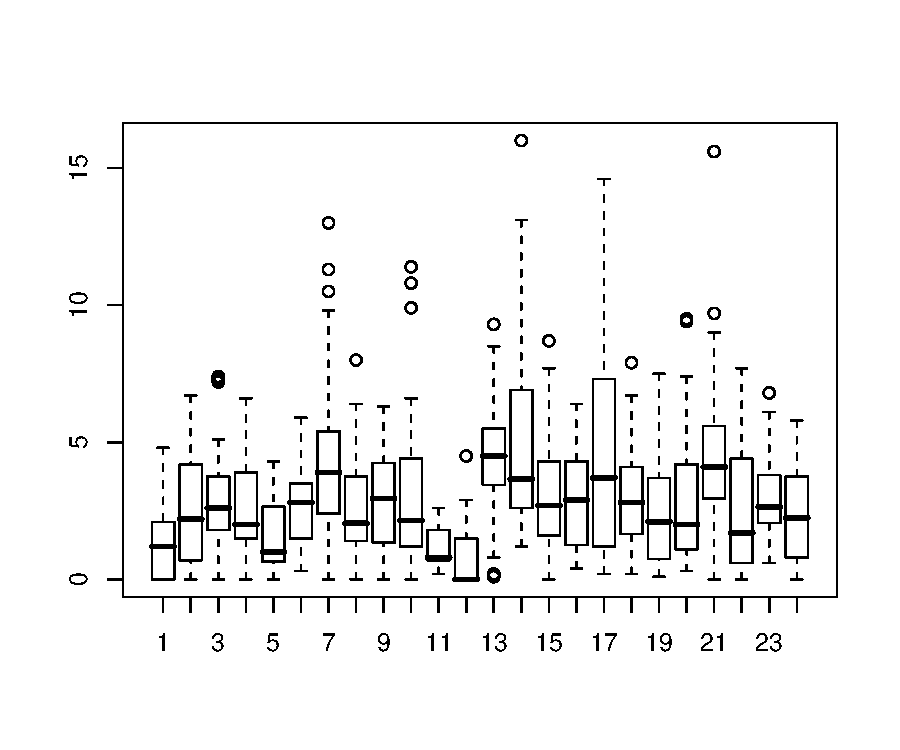
\includegraphics{Animal-007}



\begin{thebibliography}{9}
  \bibitem{cowlog} H�nninen, L. \& Pastell, M. CowLog: Open source
    software for coding behaviors from digital video. Behavior
    Research Methods. (Accepted for publication) 
\end{thebibliography}

\end{document}





